\chapter{Creating Figures}\label{Ch:creating_figures}

Example text preceding the figure command.
%
\begin{figure}%[optional modifiers]
    \centering
    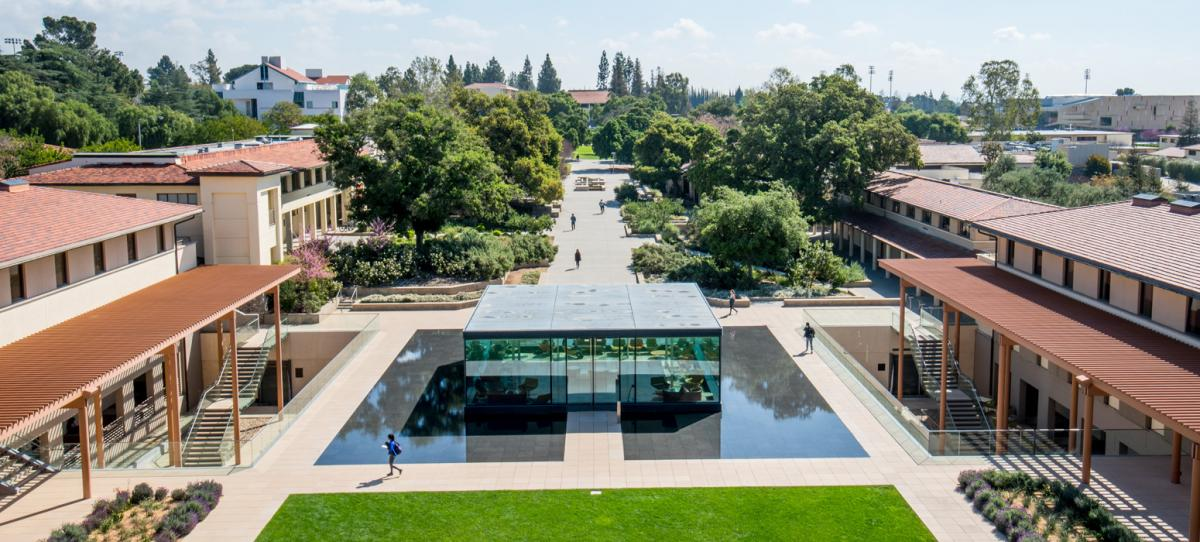
\includegraphics[width=5cm]{Graphic1.jpg}
    \qquad %For a sufficient space between side by side graphics
    
\includegraphics[width=5cm]{Graphic2.jpg}
    \caption{Very short gist of the point of this figure's inclusion. (a) Long, descriptive caption of the first graphic. (b) Long, descriptive caption of the second graphic.}
    \label{FIG_DESCRIPTIVELABEL}
\end{figure}
%
Example text post the figure command; still part of the same paragraph.

Example text for the following paragraph. Note that Latex places the figure close to where you called the command, but not exactly there. 

\begin{enumerate}
    \item Modifiers right after the begin command can change the figure location (ex. [t] can force the location at the top of a page).
    \item Make your captions descriptive enough so that someone who reads nothing else in your paper can still get the gist of the idea.
    \item EVERY figure needs to be referenced in the document and in the order in which they are presented.
    \item Plots must not depend on colors to differentiate between graphs. Alternative methods include dotted or dashed lines or identifying token at graph vertices. Using color is, of course, still welcome, but must be a supplement.
    \item All axis of a plot must be labeled with nicely readable and large fonts.
    \item If there are more than two graphics in a figure, they must each be labeled (as part of the graphic) with a letter (a), (b), (c), etc. Each graphic must be described in the caption.
\end{enumerate}





\endinput